\PassOptionsToPackage{unicode=true}{hyperref}
\documentclass[17pt]{beamer}
\usepackage[utf8]{inputenc}
\usepackage[utf8]{vietnam}
%\usetheme{CambridgeUS}
\mode<beamer>{\usetheme{CambridgeUS}}
\usepackage{utopia}
\usepackage{amsmath}
\usepackage{amsfonts}
\usepackage{amssymb}

\makeatletter
\def\verbatim@font{\footnotesize\ttfamily}
\makeatother

\usepackage{ragged2e}
\usepackage{etoolbox}
\apptocmd{\frame}{}{\justifying}{}

\author[Thi Minh Nhựt]{Thi Minh Nhựt -- thiminhnhut@gmail.com}
\title[Tiếng Việt trong Bookmark]{Hiển thị tiếng Việt vào Bookmark của PDF trong Beamer}
\date[Cần Thơ, 2016]{Ngày 10 tháng 12 năm 2016} 

\begin{document}
\begin{frame}
\titlepage
\end{frame}

%\begin{frame}
%\tableofcontents
%\end{frame}

\section{Hiển thị tiếng Việt vào Bookmark trong Beamer}
\begin{frame}[fragile]{Cách thực hiện}
	\begin{block}{Cú pháp}
		Thêm vào lệnh bên dưới trước lệnh \verb+\documentclass+
		
		\verb+\PassOptionsToPackage{unicode=true}{hyperref}+
	\end{block}
	
	Ví dụ: trạng thái bookmark trước và sau khi khai báo  lệnh \verb+\PassOptionsToPackage+.
	\begin{center}
			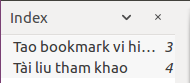
\includegraphics[scale=.61]{images/bookmark-khongtiengviet.png} \hspace{.2cm}
			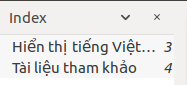
\includegraphics[scale=.6]{images/bookmark-tiengviet.png} 
		\end{center}
\end{frame}

\section{Tài liệu tham khảo}
\begin{frame}{Tài liệu tham khảo}
	\begin{enumerate}[{[1]}]
		\justifying
		\item \href{http://tex.stackexchange.com/questions/308047/option-unicode-and-beamer-with-lualatex}{Option unicode and beamer with LuaLaTeX}, \href{http://tex.stackexchange.com/}{TeX - LaTeX Stack Exchange}
		
		\item Source code \LaTeX{} của bài viết: 
		
		\href{https://github.com/h3int2um/latex/tree/master/beamer/tips-beamer/example/bookmark-tiengviet}{\footnotesize{https://github.com/h3int2um/latex/tree/master/beamer/tips-beamer/example/bookmark-tiengviet}}
	\end{enumerate}
\end{frame}
\end{document}